%!TEX root = ../main.tex
%%%%%%%%%%%%%%%%%%%%%%%%%%%%%%%%%%%%%%%%%
%
%LEZIONE 26/02/2016 - PRIMA SETTIMANA (3)
%
%%%%%%%%%%%%%%%%%%%%%%%%%%%%%%%%%%%%%%%%%
\chapter{Funzioni aritmetiche}
%%%%%%%%%%%%%%
%INTRODUZIONE%
%%%%%%%%%%%%%%
\section{Introduzione}

\begin{defn}{Funzione aritmetica}{funzioneAritmetica}\index{Funzione!aritmetica}
	Una \emph{funzione aritmetica} è un'applicazione
	\[
		f\colon \N\to\C.
	\]
\end{defn}

\begin{defn}{Funzione moltiplicativa}{funzioneMolt}
	Una funzione aritmetica si dice \emph{moltiplicativa}, se
	\[
		f(n\,m)=f(n)f(m),\,\fa n,m\in\N:(n,m)=1.
	\]
\end{defn}

\begin{defn}{Funzione totalmente moltiplicativa}{funzioneTotMolt}
	Una funzione aritmetica si dice \emph{totalmente moltiplicativa}, se
	\[
		f(n\,m)=f(n)f(m),\,\fa n,m\in\N.
	\]
\end{defn}

\begin{ese}
	\begin{itemize}
		\item \(f(n)=n^k\) è una funzione totalmente moltiplicativa.
		\item \(f(n)=1\) è una funzione totalmente moltiplicativa.
		\item \(f(n)=\ln n\) non è una funzione moltiplicativa.
		\item \(d(n)=\#\Set{d\in\N:d\mid n}\) è una funzione moltiplicativa, ma non totalmente, infatti
		      \[
			      d(p^2)=3\neq d(p)d(p)=2\cdot 2=4.
		      \]
		\item \(\s(n)\), che è la somma dei divisori di \(n\), è una funzione moltiplicativa, ma non totalmente, infatti
		      \[
			      \s(p^2)=1+p+p^2\neq\s(p)\s(p)=1+2p+p^2.
		      \]
	\end{itemize}
\end{ese}

\begin{defn}{Trasformata di Dirichlet}{trasfDirichlet}\index{Trasformata di Dirichlet}
	Sia \(f\) una funzione aritmetica, si definisce \emph{trasformata di Dirichlet} di \(f\) la seguente funzione
	\[
		g(n)=\sum_{d\mid n}f(d).
	\]
\end{defn}

\begin{teor}{La trasformata di Dirichlet è moltiplicativa}{2.1}
	Sia \(f\) una funzione moltiplicativa.
	Allora la trasformata di Dirichlet \(g\) di \(f\) è moltiplicativa.
\end{teor}

\begin{proof}
	Per l'osservazione del teorema \ref{th:1.5}, sappiamo che, presi \(n,m\in\N\) con \((n,m)=1\), si ha una corrispondenza biunivoca
	\[
		\mathcal{D}(n)\times\mathcal{D}(m)\longleftrightarrow\mathcal{D}(n\,m),
	\]
	tramite l'applicazione \((u,v)\mapsto u\,v\).

	Vogliamo mostrare che
	\[
		g(n)=\sum_{d\mid n}f(d),
	\]
	è moltiplicativa, cioè che \(g(n\,m)=g(n)g(m)\) se \((n,m)=1\).
	Ora
	\[
		\begin{split}
			g(n\,m) & =\sum_{d\mid n\,m}f(d)\\
			& =\sum_{d\in\mathcal{D}(n\,m)} f(d)\\
			& = \sum_{(u,v)\in\mathcal{D}(n)\times\mathcal{D}(m)} f(u\,v),
		\end{split}
	\]
	ma \((n,m)=1\), quindi \((u,v)=1\), ovvero
	\[
		f(u\,v)=f(u)f(v),
	\]
	per la molteplicità di \(f\).
	Per cui
	\[
		\begin{split}
			\sum_{(u,v)\in\mathcal{D}(n)\times\mathcal{D}(m)} f(u\,v) & =\sum_{u\in\mathcal{D}(n)}\sum_{v\in\mathcal{D}(m)}f(u)f(v)\\
			& =\sum_{u\in\mathcal{D}(n)}f(u)\sum_{v\in\mathcal{D}(m)}f(v)\\
			& =g(n)g(m).\qedhere
		\end{split}
	\]
\end{proof}

\begin{cor}
	La funzione
	\[
		d(n)=\#\Set{d\in\N:d\mid n},
	\]
	è moltiplicativa.
\end{cor}

\begin{proof}
	Dalla definizione di \(d\) segue che
	\[
		d(n)=\sum_{d\mid n}1,
	\]
	ovvero \(d\) è la trasformata di Dirichlet della funzione \((n)=1\), la quale è banalmente moltiplicativa.
\end{proof}

\begin{cor}
	La funzione \(\s(n)\), somma dei divisori di \(n\), è moltiplicativa.
\end{cor}

\begin{proof}
	Dalla definizione di \(\s\) segue che
	\[
		\s(n)=\sum_{d\mid n} d,
	\]
	ovver \(\s\) è la trasformata di Dirichlet della funzione identità \(id(n)=n\), che è moltiplicativa.
\end{proof}

\begin{oss}
	Supponiamo che \(f\) sia moltiplicativa, allora
	\begin{itemize}
		\item Se \(f\) non è la funzione nulla, \(f(1)=1\), infatti, preso \(a\in\N\) tale che \(f(a)\neq 0\), si avrà
		      \[
			      f(a)=f(a\cdot 1)=f(a)f(1),
		      \]
		      ovvero \(f(1)=1\).
		\item \(f(p_1^{\a_1}\cdot\ldots\cdot p_s^{\a_s})=f(p_1^{\a_1})\ldots f(p_s^{\a_s})\), con \(p_1<p_2<\ldots<p_s\), ovvero
		      \[
			      f(n)=\prod_p f(p^{v_p(n)}).
		      \]
	\end{itemize}
\end{oss}

\begin{prop}{Scrittura alternativa delle funzioni enumerativa e somma dei divisori}{2.2}
	Sia \(n=p_1^{\a_1}\cdot\ldots\cdot p_s^{\a_s}\), allora
	\[
		d(n)=\prod_{j=1}^s (\a_j+1)\text{ e }\s(n)=\prod_{j=1}^s \frac{p_j^{a_j+1}-1}{p_j-1}.
	\]
\end{prop}
\begin{proof}
	Segue dalla molteplicità di \(d\) e di \(\s\), infatti
	\[
		\begin{split}
			d(p_1^{\a_1}\cdot\ldots\cdot p_s^{\a_s}) & =d(p_1^{\a_1})\ldots d(p_s^{\a_s})\\
			& =\prod_{j=1}^s (\a_j+1).
		\end{split}
	\]
	Analogamente
	\[
		\begin{split}
			\s(p_1^{\a_1}\cdot\ldots\cdot p_s^{\a_s}) & =\s(p_1^{\a_1})\ldots\s(p_s^{\a_s})\\
			& =\prod_{j=1}^s\sum_{k=0}^{\a_j}p_j^k\\
			& =\prod_{j=1}^s\frac{p_j^{a_j+1}-1}{p_j-1}.\qedhere
		\end{split}
	\]
\end{proof}
%%%%%%%%%%%%%%%%%%%%%%%%%%%%%%%%%%%%%%%%%%%
%
%LEZIONE 26/02/2016 - SECONDA SETTIMANA (1)
%
%%%%%%%%%%%%%%%%%%%%%%%%%%%%%%%%%%%%%%%%%%%
%%%%%%%%%%%%%%%%%
%NUMERI PERFETTI%
%%%%%%%%%%%%%%%%%
\section{Numeri perfetti}

\begin{defn}{Numero perfetto}{numPerfetto}\index{Numero!perfetto}
	Un numero naturale \(n\) si definisce \emph{perfetto} se
	\[
		\s(n)=2n.
	\]
\end{defn}

\begin{oss}
	I numeri primi non sono mai perfetti, infatti
	\[
		\s(p)=1+p\neq 2p,\,\fa p\text{ primo}.
	\]
	Osserviamo che vale anche \(\s(n)=1+n\implies n\) primo, questo poichè, se per assurdo \(n=a\,b\), dove \(a,b\) sono divisori propri di \(n\), si avrebbe
	\[
		\s(n)\ge n+1+a+b\neq n+1.
	\]
\end{oss}

\begin{ese}
	\(6\) è un numero perfetto, infatti
	\[
		\s(6)=\s(2)\s(3)=3\cdot 4=12=2\cdot 6.
	\]
	Anche \(28\) è un numero perfetto, infatti
	\[
		\s(28)=\s(4)\s(7)=7\cdot 8=56=2\cdot 28.
	\]
\end{ese}

\begin{teor}{Numeri perfetti pari}{2.4}
	Sia \(n\in\N\) pari.
	Allora \(n\) è perfetto se e soltanto se
	\[
		n=2^{m-1}(2^m-1),\text{ con }2^m-1\text{ primo}.
	\]
\end{teor}

\begin{proof}
	\graffito{\(\Leftarrow)\) dovuta a Euclide}Supponiamo che
	\[
		n=2^{m-1}(2^m-1),
	\]
	con \(2^m-1\) primo, allora
	\[
		\begin{split}
			\s(n) & =\s(2^{m-1})\s(2^m-1)\\
			& =(1+2+\ldots+2^{m-1})(2^m-1+1)\\
			& =(2^m-1)2^m\\
			& =2n,
		\end{split}
	\]
	dove la penultima uguaglianza discende da
	\[
		\sum_{n=0}^k a^n=\frac{a^{k+1}-1}{a-1}\overset{a=2}{=}2^{k+1}-1.
	\]

	\graffito{\(\Rightarrow)\) dovuta a Eulero}Sia \(n\) un numero perfetto pari, per cui
	\[
		n=2^{m-1}u,
	\]
	dove \(u\) è dispari e \(m>1\).
	Ora, \(n\) è perfetto, quindi \(2n=\s(n)\), da cui
	\[
		2^m u=\s(2^{m-1})\s(u)=(2^m-1)\s(u),
	\]
	ovvero
	\[
		\begin{split}
			\s(u) & =\frac{2^m u}{2^m-1}\\
			& =\frac{2^m u-u+u}{2^m-1}\\
			& =u+\frac{u}{2^m-1},
		\end{split}
	\]
	quindi
	\[
		\frac{u}{2^m-1}=\s(u)-u\in \N\graffito{ricordiamo che \((1+u)\le\s(u)\)}
	\]
	per cui
	\[
		2^{m-1}\mid u\implies \frac{u}{2^m-1}\mid u.\graffito{\(a\mid b\implies \frac{b}{a}a=b\implies \frac{b}{a}\mid b\)}
	\]
	Quindi sappiamo che
	\[
		\s(u)=u+\frac{u}{2^m-1},
	\]
	che sono entrambi divisori di \(u\).
	Ricordiamo che \(\s(u)\) è la somma dei divisori di \(u\) e che \(\s(u)\ge u+1\).
	Per cui avremo necessariamente
	\[
		u+1=u+\frac{u}{2^m-1},
	\]
	ovvero
	\[
		u=2^m-1.\qedhere
	\]
\end{proof}

\begin{oss}
	In generale basta trovare un primo della forma \(2^m-1\) per avere un numero perfetto.
\end{oss}

\begin{ese}
	Alcuni numeri perfetti trovati tramite il teorema:
	\begin{itemize}
		\item \(2\cdot 3=6\);
		\item \(2^2(2^3-1)=28\);
		\item \(2^4(2^5-1)=16\cdot 31=496\).
	\end{itemize}
\end{ese}

\begin{defn}{Numero primo di Mersenne}{numMersenne}\index{Numero!primo di Mersenne}
	Un numero primo della forma
	\[
		2^m-1,
	\]
	si definisce \emph{numero primo di Mersenne}.
\end{defn}

\begin{oss}
	Si conoscono solamente \(49\) primi di Mersenne e non è stato dimostrato se sono o meno infiniti.
	Il più grande conosciuto è, ad oggi,
	\[
		2^{74207281}-1,
	\]
	che ha più di \(22\) milioni di cifre.
\end{oss}

\begin{pr*}
	\[
		2^n-1\text{ primo}\implies n\text{ primo}.
	\]
\end{pr*}

\begin{proof}
	Se per assurdo \(n=a\,b\), con \(a,b\) divisori propri di \(n\), si avrebbe
	\[
		\begin{split}
			2^n-1 & =2^{a\,b}-1\\
			& =(2^a-1)(1+2^a+2^{2a}+\ldots+2^{(b-1)a}),
		\end{split}
	\]
	che è una fattorizzazione propria di \(2^n-1\) se \(a>1\).
	Ma ciò è assurdo in quanto avevamo supposto che \(2^n-1\) fosse primo.
\end{proof}

\begin{oss}
	Fino ad oggi non è stato dimostrato se esistono o meno numeri perfetti dispari, di seguito andremo a mostrare alcuni risultati in questo ambito.
\end{oss}

\begin{pr*}
	Se \(n\) è un numero perfetto dispari, allora
	\begin{itemize}
		\item \(n>10^{1500}\);
		\item il più grande dei suoi divisori primi è maggiori di \(10^8\).
	\end{itemize}
\end{pr*}

\begin{pr*}[Teorema di Eulero]
	Se \(n\) è un numero perfetto dispari, allora
	\[
		n=p^{4\l+1}Q^2,
	\]
	dove \(p=1+4k\) e \(Q^2\) è un quadrato perfetto.
\end{pr*}
%%%%%%%%%%%%%%%%%%%%%%%%%%
%LA FUNZIONE DEI DIVISORI%
%%%%%%%%%%%%%%%%%%%%%%%%%%
\section{La funzione dei divisori}

\begin{defn}{Notazione di Vinogradov}{notzVinogradov}\index{Notazione!di Vinogradov}
	Prese due funzioni aritmetiche \(f,g\), diremo che
	\[
		f\ll g,\text{ per }n\to+\infty,
	\]
	se esistono \(A,B\) costanti tali che
	\[
		\frac{\abs{f(n)}}{\abs{g(n)}}\le A,\,\fa n\ge B.
	\]
\end{defn}

\begin{oss}
	\(f\ll g\iff f=O(g)\).
\end{oss}

\begin{teor}{Stima superiore della funzione dei divisori}{2.6}
	Preso \(\e>0\) qualsiasi, risulta
	\[
		d(n)\ll n^\e,\text{ per }n\to+\infty.
	\]
\end{teor}

\begin{proof}
	Fissiamo \(\e>0\) e, senza perdita di generalità, assumiamo che \(\e<1\).
	Sia \(n=p_1^{\a_1}\cdot\ldots\cdot p_s^{\a_s}\), avremo
	\[
		\frac{d(n)}{n^\e}=\frac{\a_1+1}{p_1^{\a_1\e}}\cdot\ldots\cdot\frac{\a_s+1}{p^{\a_s\e}},
	\]
	vogliamo stimare ciascun fattore.
	Avremo quindi due casi:
	\begin{itemize}
		\item Se \(2\le p_j\le 2^{\frac{1}{\e}}\), avremo
		      \[
			      2^{\a_j\e}\le p_j^{\a_j\e}\le 2^{\a_j},
		      \]
		      da cui
		      \[
			      \frac{\a_j+1}{p_j^{\a_j\e}}\le\frac{\a_j+1}{2^{\a_j\e}}.
		      \]
		      Ora
		      \[2^{a_j\e}\ge 1+\e\,\a_j\ln 2,
		      \]
		      in quanto, per Taylor,
		      \[
			      2^{\a_j\e}=e^{\a_j\e\ln 2}=1+\e\,\a_j\ln 2+o(\e\,\a_j\ln 2).
		      \]
		      Infine
		      \[
			      1+\e\,\a_j\ln 2> (1+\a_j)\e\ln 2,
		      \]
		      è vero poichè
		      \[
			      \e\ln 2<1\iff \e<\frac{1}{\ln 2},
		      \]
		      che è soddisfatta in quanto \(\e<1\).
		      Per cui avremo
		      \[
			      \frac{\a_j+1}{p^{\a_j\e}}<\frac{1}{\e\ln 2}.
		      \]
		\item Se \(p_j>2^{\frac{1}{\e}}\), avremo
		      \[
			      p_j^{\a_j\e}>2^{a_j}>1+\a_j,
		      \]
		      dove l'ultima disuguaglianza è vera poichè
		      \[
			      \begin{split}
				      2^\a & =(1+1)^\a\\
				      & =\sum_{k=0}^\a \binom{\a}{k}\\
				      & >\binom{\a}{0}+\binom{\a}{1}\\
				      & =1+\a.
			      \end{split}
		      \]
		      Per cui avremo
		      \[
			      \frac{\a_j+1}{p_j^{\a_j\e}}<1.
		      \]
	\end{itemize}
	Concludendo, abbiamo che
	\[
		\frac{d(n)}{n^\e}=\prod_{j=1}^s\frac{\a_j+1}{p_j^{\a_j\e}}<\prod_{\substack{j=1\\p_j<2^{1/\e}}}\frac{1}{\e\ln 2},
	\]
	da cui
	\[
		\begin{split}
			\frac{d(n)}{n^\e} & \le\prod_{\substack{i=1\\p_j\le2^{1/\e}}}\frac{1}{\e\ln 2}\\
			& \le\prod_{p\le2^{1/\e}}\frac{1}{\e\ln 2}\graffito{\(p\) è un generico primo indipendente da \(n\)}\\
			& =K_\e,
		\end{split}
	\]
	che è un valore indipendente da \(n\).
	Abbiamo quindi ottenuto
	\[
		\frac{d(n)}{n^\e}\le K_\e,
	\]
	cioè \(d(n)\ll n^\e\).
\end{proof}
%%%%%%%%%%%%%%%%%%%%%%%%%%%%%%%%%%%%%%%%%%%
%
%LEZIONE 03/02/2016 - SECONDA SETTIMANA (2)
%
%%%%%%%%%%%%%%%%%%%%%%%%%%%%%%%%%%%%%%%%%%%
\begin{ese}
	Se prendiamo \(\e=\frac{1}{3}\), avremo
	\[
		K_{\frac{1}{3}}=\prod_{p\le 8}\frac{3}{\ln 2}=\left(\frac{3}{\ln 2}\right)^4,
	\]
	per cui
	\[
		\frac{d(n)}{n^{\frac{1}{3}}}<\left(\frac{3}{\ln 2}\right)^4.
	\]
\end{ese}

\begin{teor}{Impossibilità di stimare meglio la funzione dei divisori}{2.5}
	Preso \(c\in\R^+\), la disuguaglianza
	\[
		d(n)\ll \ln^c n,\text{ per }n\to+\infty,
	\]
	è falsa.
\end{teor}

\begin{proof}
	Fissiamo \(c\), la strategia è cotruire una sequenza di numeri infinita, tale che
	\[
		d(n)>k\ln n,\,\fa k>0.
	\]
	Fissiamo \(l=[c]\), la sequenza è la seguente
	\[
		n=(p_1 p_2\cdot\ldots\cdot p_{l+1})^m,m\in\N,
	\]
	dove \(p_i\) è l'i-esimo numero primo.\graffito{ovvero \(p_1=2,p_2=3\), ecc.}
	Ora \(d(n)=(m+1)^{l+1}\), e \(\ln n=m\ln(p_1\cdot\ldots\cdot p_{l+1})\), da cui
	\[
		\begin{split}
			d(n) & =(m+1)^{l+1}\\
			& >m^{l+1}\\
			& =m^{l+1}\frac{\big(\ln(p_1\cdot\ldots\cdot p_{l+1})\big)^{l+1}}{\big(\ln(p_1\cdot\ldots\cdot p_{l+1})\big)^{l+1}}\\
			& =\frac{1}{\big(\ln(p_1\cdot\ldots\cdot p_{l+1})\big)^{l+1}}(\ln n)^{l+1}\\
			& >k (\ln n)^c,
		\end{split}
	\]
	dove l'ultima uguaglianza è vera se e soltanto se
	\[
		(\ln n)^{l+1-c}>k\big(\ln(p_1\cdot\ldots\cdot p_{l+1})\big)^{l+1},
	\]
	che è soddisfatta per ogni \(n\) sufficientemente grande.
\end{proof}

\begin{defn}{Costante di Eulero-Mascheroni}{costEuleroMascheroni}\index{Costante!di Eulero-Mascheroni}
	La \emph{costante di Eulero-Mascheroni} \(\g\) è definita come il limite della differenza tra la serie armonica troncata e il logaritmo naturale,
	\[
		\g=\lim_{n\to+\infty}\left(\sum_{k=1}^n \frac{1}{k}-\ln n\right).
	\]
\end{defn}

\begin{oss}
	La costante di Eulero-Mascheroni converge, in particolare
	\[
		\g\simeq 0,577215649\dots
	\]
\end{oss}

\begin{teor}{Stima asintotica della serie armonica tramite \(\g\)}{2.8}
	Vale la seguente stima
	\[
		\sum_{n\le Y}\frac{1}{n}=\ln Y+\g+O\left(\frac{1}{Y}\right),\text{ con }Y\to+\infty.
	\]
\end{teor}

\begin{proof}
	Preso \(Y\ge 1,Y\in \R\), vale la seguente identità
	\[
		\sum_{n\le Y}\frac{1}{n}=\frac{[Y]}{Y}+\int_1^Y \frac{[u]}{u^2}\,\dd u,
	\]
	infatti
	\[
		\begin{split}
			\frac{[Y]}{Y}+\int_1^Y \frac{[u]}{u^2}\,\dd u & =\frac{[Y]}{Y}+\sum_{n=1}^{[Y]-1}\int_n^{n+1}\frac{[u]}{u^2}\,\dd u+\int_{[Y]}^Y \frac{[u]}{u^2}\,\dd u\\
			& =\frac{[Y]}{Y}+\sum_{n=1}^{[Y]-1} n \int_n^{n+1}\frac{\dd u}{u^2}+ [Y]\int_{[Y]}^Y \frac{\dd u}{u^2}\\
			& =\frac{[Y]}{Y}+\sum_{n=1}^{[Y]-1}n\left(\frac{1}{n}-\frac{1}{n+1}\right)+[Y]\left(\frac{1}{[Y]}-\frac{1}{Y}\right)\\
			& =\sum_{n=1}^{[Y]-1}\frac{1}{n+1}+1\\
			& =1+\frac{1}{2}+\frac{1}{3}+\ldots+\frac{1}{[Y]}\\
			& =\sum_{n\le Y}\frac{1}{n}.
		\end{split}
	\]
	Da cui
	\[
		\begin{split}
			\sum_{n\le Y}\frac{1}{n} & =\frac{[Y]}{Y}+\int_1^Y \frac{[u]}{u^2}\,\dd u\\
			& =\frac{[Y]}{Y}+\int_1^Y \frac{u-\{u\}}{u^2}\,\dd u\\
			& =1-\frac{\{Y\}}{Y}+\ln Y-\int_1^Y \frac{\{u\}}{u^2}\,\dd u\\
			& =1-\int_1^{+\infty}\frac{\{u\}}{u^2}\,\dd u+\ln Y-\frac{\{Y\}}{Y}+\int_Y^{+\infty}\frac{\{u\}}{u^2}\,\dd u.
		\end{split}
	\]
	Sia quindi
	\[
		\g=1-\int_1^{+\infty}\frac{\{u\}}{u^2}\,\dd u,
	\]
	dove
	\[
		\int_1^{+\infty}\frac{\{u\}}{u^2}\,\dd u \le \int_1^{+\infty}\frac{\dd u}{u^2}=1,
	\]
	che implica \(\g\in \R\) e \(\g\ge 0\).
	Sia inoltre
	\[
		E(Y)=\int_Y^{+\infty}\frac{\{u\}}{u^2}\,\dd u-\frac{\{Y\}}{Y}.
	\]
	Avremo quindi
	\[
		\sum_{n\le Y}\frac{1}{n}=\ln Y+\g+E(Y).
	\]
	Resta da mostrare che \(E(Y)\ll \frac{1}{Y}\), infatti
	\[
		\begin{split}
			\abs{E(Y)} & \le \int_Y^{+\infty}\frac{\dd u}{u^2}+\frac{1}{Y}\\
			& =\left.-\frac{1}{u}\right|_Y^{+\infty}+\frac{1}{Y}\\
			& =\frac{2}{Y}\\
			& =O\left(\frac{1}{Y}\right).\qedhere
		\end{split}
	\]
\end{proof}

\begin{teor}{dell'iperbole di Dirichlet}{2.7}\index{Teorema!dell'iperbole di Dirichlet}
	Vale la seguente stima
	\[
		\sum_{n\le X}d(n)=\ln X+(2\g-1)X+O\big(\sqrt{X}\big),\text{ con }X\to+\infty.
	\]
\end{teor}

\begin{proof}
	Sappiamo che
	\[
		d(n)=\sum_{d\mid n}1,
	\]
	per cui
	\[
		\sum_{n\le X}d(n)=\sum_{n\le X}\sum_{d\mid n}1=\sum_{\substack{a,b\in\N\\a\,b\le X}}1,
	\]
	questo poichè esiste un corrispondenza biunivoca
	\[
		\Set{(a,b)\in \N | a\, b\le X}\longleftrightarrow \Set{(n,d)\in\N:n\le X,d\mid n},
	\]
	tramite le applicazioni
	\begin{gather*}
		(a,b)\mapsto(a\,b,a),\\
		\left(d,\frac{n}{d}\right)\mapsfrom (n,d).
	\end{gather*}
	Ora, come mostrato nella figura \ref{fig:2.7}, \(\sum_{a\,b\le X}1\) è il numero di punti a coordinate intere che si trovano al di sotto dell'iperbole \(a\,b=X\).
	Preso il punto \(P=(\sqrt{X},\sqrt{X})\), posso quindi considerare tale superficie suddivisa come nelle tre regioni in figura.
	Avrò quindi
	\[
		\sum_{\substack{a,b\in\N\\a\,b\le X}}1 =I+II-III=2I-III = 2\sum_{a\le\sqrt{X}}\sum_{b\le\frac{X}{a}}1-\big([\sqrt{X}]\big)^2\graffito{in \(III\) ho precisamente \([\sqrt{X}]\) punti di \(b\) per ognuno dei \([\sqrt{X}]\) punti di \(a\)},
	\]
	da cui
	\[
		\begin{split}
			\sum_{n\le X}d(n) & =2\sum_{a\le \sqrt{X}}\left[\frac{X}{a}\right]-\big(\sqrt{X}-\{\sqrt{X}\}\big)^2\graffito{applico la proprietà \(9\) della parte intera}\\
			& =2\sum_{a\le\sqrt{X}}\frac{X}{a}-\underbrace{2\sum_{a\le \sqrt{X}}\overbrace{\left\{\frac{X}{a}\right\}}^{\le 1}}_{\le 2\sqrt{X}}-X+\underbrace{2\{X\}\sqrt{X}}_{\le2\sqrt{X}}-\underbrace{\{X\}^2}_{\le 1}\\
			& =2X\sum_{a\le \sqrt{X}}\frac{1}{a}-X+O\big(\sqrt{X}\big)\\
			& =2X\left[\ln\sqrt{X}+\g+O\left(\frac{1}{\sqrt{X}}\right)\right]-X+O\big(\sqrt{x}\big)\graffito{la stima della serie armonica viene dal teorema precedente}\\
			& =X\ln X+(2\g-1)X+O\big(\sqrt{X}\big).\qedhere
		\end{split}
	\]
\end{proof}
%%%%%%%%%%%%%%%%%%%%%%%%%%%%%%%%%%%%%%%%%%%
%
%LEZIONE 04/03/2016 - SECONDA SETTIMANA (3)
%
%%%%%%%%%%%%%%%%%%%%%%%%%%%%%%%%%%%%%%%%%%%
\begin{figure}[tp]
	\begin{centering}
		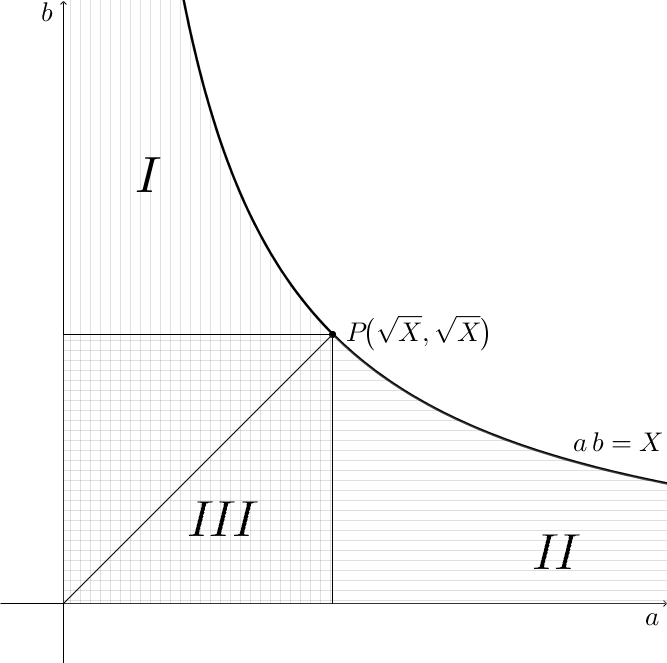
\includegraphics{fig1.png}
		\caption{La porzione di piano sottesa da \(a\,b=X\), suddivisa in \(3\) regioni.}
		\label{fig:2.7}
	\end{centering}
\end{figure}

\begin{oss}
	Un risultato molto più debole
	\[
		\sum_{n\le X} d(n)=X\ln X+O(X),
	\]
	può essere ottenuto più facilmente troncando il secondo termine significativo, infatti
	\[
		\begin{split}
			\sum_{n\le X}\sum_{d\mid n}1 & =\sum_{d\le X}\sum_{\substack{n\le X\\d\mid n}}1\\
			& =\sum_{d\le X}\left[\frac{X}{d}\right]\\
			& =\sum_{d\le X}\frac{X}{d}-\underbrace{\sum_{d\le X}\left\{\frac{X}{d}\right\}}_{\le X=O(X)}\\
			& =X\sum_{d\le X}\frac{1}{d}+O(X)\\
			& =X\left[\ln X+\g+O\left(\frac{1}{X}\right)\right]+O(X)\\
			& =X\ln X+\g X+O(1)+O(X)\graffito{i termini \(O(1)\) e \(\g X\) vengono inglobati da \(O(X)\)}\\
			& =X\ln X+O(X).
		\end{split}
	\]
\end{oss}

\begin{oss}
	Esiste una congettura, equivalente all'ipotesi di Riemann, che stima l'errore di
	\[
		\sum_{n\le X}d(n),
	\]
	come \(O\big(X^{1/4}\big)\).
\end{oss}

\begin{teor}{Stima superiore della funzione somma dei divisori}{2.9}
	Consideriamo la funzione somma dei divisori \(\s\), allora
	\[
		\s(n)\ll n\ln n.
	\]
\end{teor}

\begin{proof}
	Osserviamo che l'applicazione
	\[
		\mathcal{D}(n)\to\mathcal{D}(n),d\mapsto\frac{n}{d},
	\]
	è un involuzione, ovvero è un applicazione biunivoca che ha se stessa come inversa.
	Da cui
	\[
		\s(n)=\sum_{d\mid n}d=\sum_{d\mid n}\frac{n}{d}.
	\]
	Segue
	\[
		\begin{split}
			\s(n) & =\sum_{d\mid n}\frac{n}{d}\\
			& =n\sum_{d\mid n}\frac{1}{d} \le n\sum_{d\le n}\frac{1}{d}\\
			& =n\left[\ln n+\g+O\left(\frac{1}{b}\right)\right] \le 2n\ln n,
		\end{split}
	\]
	quando \(n\) è sufficientemente grande.
	Ovvero \(\s(n)\ll n\ln n\).
\end{proof}

\begin{teor}{Stima asintotica della funzione somma dei divisori}{2.10}
	Consideriamo la funzione somma dei divisori \(\s\), allora
	\[
		\sum_{n\le X}\s(n)=\frac{\p^2}{12}X^2+O(X\ln X).
	\]
\end{teor}

\begin{proof}
	Per definizione di \(\s\) avremo
	\[
		\begin{split}
			\sum_{n\le X}\s(n) & =\sum_{n\le X}\sum_{d\mid n}d = \sum_{n\le X}\sum_{d\mid n}\frac{n}{d}\graffito{vedi la dimostrazione del teorema precedente}\\
			& =\sum_{d\le X}\sum_{\substack{n\le X\\d\mid n}}\frac{d}{n} = \sum_{d\le X}\sum_{m\le \frac{X}{d}}m,
		\end{split}
	\]
	dove l'ultima uguaglianza è vera in quanto \(d\mid n\) implica \(n=m\,d\), inoltre \(n\le X\), da cui
	\[
		m=\frac{n}{d}\le \frac{X}{d}.
	\]
	Ricordiamo la ben nota formula per la somma dei primi \(N\) numeri interi
	\[
		\sum_{k=1}^N k=\frac{N(N+1)}{2},
	\]
	da cui
	\[
		\begin{split}
			\sum_{d\le X}\sum_{m\le\frac{X}{d}}m & =\sum_{d\le X}\frac{1}{2}\left[\frac{X}{d}\right]\left(\left[\frac{X}{d}\right]+1\right)\\
			& =\frac{1}{2}\sum_{d\le X}\left(\frac{X}{d}+O(1)\right)\left(\frac{X}{d}+O(1)\right)=\frac{1}{2}\sum_{d\le X}\left(\frac{X^2}{d^2}+O\left(\frac{X}{d}\right)\right)\\
			& =\frac{X^2}{2}\sum_{d\le X}\frac{1}{d^2}+O\underbrace{\left(X\sum_{d\le X}\frac{1}{d}\right)}_{\ll X\ln X}\graffito{per il teorema precedente}\\
			& =\frac{X^2}{2}\sum_{d=1}^{+\infty}\frac{1}{d^2}+O(X\ln X)-\frac{X^2}{2}\left(\sum_{d>X}\frac{1}{d^2}\right).
		\end{split}
	\]
	Ricordiamo il criterio del confronto integrale per serie:
	\[
		\int_1^X f(t)\,\dd t\ll \sum_{n=1}^X f(n) \ll \int_1^X f(t)\,\dd t,
	\]
	dove \(f\) è continua e \(f\ge 0\).
	Quindi
	\[
		\sum_{d\ge X}\frac{1}{d^2}\ll \int_X^{+\infty}\frac{\dd t}{t^2}=\frac{1}{X},
	\]
	ovvero
	\[
		\frac{X^2}{2}\left(\sum_{d\ge X}\frac{1}{d^2}\right)=O\left(X^2\frac{1}{X}\right)=O(X),
	\]
	infine, dal momento che il termine \(O(X)\) viene inglobato da \(O(X\ln X)\), avremo
	\[
		\begin{split}
			\sum_{n\le X}\s(n) & =\frac{X^2}{2}\sum_{d=1}^{+\infty}\frac{1}{d^2}+O(X\ln X)\\
			& =\frac{\p^2}{12}X^2+O(X\ln X).\qedhere
		\end{split}
	\]
\end{proof}
%%%%%%%%%%%%%%%%%%%%%%%%%%%%%%%%%%%%%%%%%
%
%LEZIONE 08/03/2016 - TERZA SETTIMANA (1)
%
%%%%%%%%%%%%%%%%%%%%%%%%%%%%%%%%%%%%%%%%%
%%%%%%%%%%%%%%%%%%%%%
%FUNZIONE DI MOEBIUS%
%%%%%%%%%%%%%%%%%%%%%
\section{Funzione di M\"oebius}

\begin{defn}{Funzione di M\"oebius}{funzioneMoebius}\index{Funzione!di M\"oebius}
	Si definisce \emph{funzione di M\"oebius} la seguente funzione aritmetica
	\[
		\m(n)=
		\begin{cases}
			1      & \text{se }n=1                            \\
			(-1)^s & \text{se }n=p_1\cdot\ldots\cdot p_s      \\
			0      & \text{se \(n\) ha un fattore quadratico}
		\end{cases}
	\]
\end{defn}

\begin{oss}
	Dire che \(n\) ha fattori moltiplicativi, significa affermare che esiste \(p\) primo tale che
	\[
		p^2 \mid n.
	\]
\end{oss}

\begin{teor}{\(\m\) è moltiplicativa}{2.11}
	La funzione \(\m\) di M\"oebius è moltiplicativa.
\end{teor}

\begin{proof}
	Siano \(n,m \in \N:(n,m)=1\), dobbiamo mostrare che \(\m(m\,n)=\m(m) \m(n)\).
	D'altronde se \(\m(m)\m(n)=0\) certamente esisterà un primo \(p\) tale che \(p^2\) divide \(n\) oppure \(m\), in entrambi i casi
	\[
		\ex p^2 \mid n\,m \implies \m(n\,m)=0.
	\]
	Se, invece, \(\m(n)\m(m) \neq 0\) avremo due possibilità
	\begin{itemize}
		\item \(n=1\) o \(m=1\), da cui segue banalmente la tesi;
		\item \(n \neq 1\) e \(m \neq 1\), quindi, per definizione di \(\m\)
		      \begin{gather*}
			      n = p_1 \cdot\ldots\cdot p_s,\\
			      m = q_1 \cdot\ldots\cdot q_r,
		      \end{gather*}
		      quindi \(\m(n) = (-1)^s\) e \(\m(m) = (-1)^r\).
		      Inoltre \(\m(n\,m) = (-1)^{r+s}\) in quanto \((n,m)=1\) implica che \(p_i \neq q_j,\,\fa i,j\).
	\end{itemize}
\end{proof}

\begin{oss}
	\(\m\) non è totalmente moltiplicativa, infatti
	\[
		1 = \m(2)\m(2) \neq \m(4) = 0.
	\]
\end{oss}

\begin{teor}{Trasformata di Dirichlet di \(\m\)}{2.12}
	La trasformate di Dirichlet di \(\m\) è
	\[
		\sum_{d\mid n}\m(d)=
		\begin{cases}
			1 & n=1     \\
			0 & n\neq 1
		\end{cases}
	\]
\end{teor}

\begin{proof}
	Ricordiamo che per il teorema \ref{th:2.1} la trasformata di Dirichlet di una funzione moltiplicativa è a sua volta moltiplicativa, quindi
	\[
		g(n)=\sum_{d\mid n}\m(d),
	\]
	è moltiplicativa in \(n\).
	Ora
	\[
		g(1)=\sum_{d\mid 1}\m(d)=\m(1)=1,
	\]
	inoltre, se \(\a \ge 1\),
	\[
		g(p^\a)=\sum_{d\mid p^\a}\m(d)=\sum_{\b=0}^\a \m(p^\b)=1-1=0.
	\]
	Infine, per la moltiplicatività di \(g\), avremo
	\[
		\begin{split}
			g(n) & =g \big( p_1^{\alpha_1}\cdot \ldots \cdot p_s^{\alpha_s} \big)\\
			& =g \big( p_1^{\a_1} \big) \cdot \ldots \cdot g \big( p_s^{\a_s} \big)\\
			& =0.\qedhere
		\end{split}
	\]
\end{proof}

\begin{teor}{Prima legge di inversione di M\"oebius}{2.13}
	Sia \(f\colon \N\to\C\) una funzione aritmetica.
	Sia \(g\colon \N\to\C\) la trasformata di Dirichlet di \(f\), allora
	\[
		g(n)=\sum_{d\mid n}f(d) \implies f(n)=\sum_{d\mid n}\mu(d) g\!\left( \frac{n}{d}\right).
	\]
\end{teor}

\begin{proof}
	Ricordiamo che esiste una corrispondenda biunivoca dell'inisieme dei divisori di \(n\) in se stesso tramite \(d\mapsto \frac{n}{d}\), per cui
	\[
		\begin{split}
			\sum_{d\mid n}\m(d) g\!\left( \frac{n}{d} \right) & =\sum_{d\mid n}\m \left( \frac{n}{d} \right) g(d)\\
			& =\sum_{d\mid n}\m \left( \frac{n}{d} \right) \sum_{e\mid d} f(e)\graffito{\(e\mid d,d\mid n\implies e\mid n\)}\\
			& =\sum_{e\mid n}f(e)\sum_{\substack{d\mid n\\e\mid d}}\m \left( \frac{n}{d} \right),
		\end{split}
	\]
	dove \(e,n\) sono fissati, inoltre \(n=d\, f,d=e\,k\), per cui
	\[
		f=\frac{n}{d}=\frac{n}{e\,k}\implies f\mid \frac{n}{e}.
	\]
	In conclusione
	\[
		\sum_{\substack{d\mid n\\e\mid d}}\m \left( \frac{n}{d} \right) =\sum_{f\mid \frac{n}{e}}\m(f)=
		\begin{cases}
			1 & e=n               \\
			0 & \text{altrimenti}
		\end{cases}
	\]
	ovvero
	\[
		\sum_{e\mid n}f(e)\sum_{\substack{d\mid n\\e\mid d}}\m \left( \frac{n}{d} \right) =f(n).
	\]
\end{proof}

\begin{ese}\label{es:z_f}
	Consideriamo la funzione \(\zeta\) di Riemann
	\[
		\zeta(s)=\sum_{n=1}^{+\infty}\frac{1}{n^s},s>1\graffito{in generale \(s\in\C\) con \(\Re(s)>1\)}
	\]
	e consideriamo
	\[
		F(s)=\sum_{n=1}^{+\infty}\frac{\m(n)}{n^s},
	\]
	dove \(\abs{\m(s)}\in\{0,1\}\), per cui \(F(s)\) converge totalmente per la convergenza di \(\zeta(s)\) quando \(s>1\).

	Facciamo il prodotto tra le due funzioni
	\[
		\sum_{n=1}^{+\infty}\frac{1}{n^s} \sum_{m=1}^{+\infty}\frac{\m(m)}{m^s} = \sum_{\substack{n\in\N\\m\in\N}}\frac{\m(m)}{(m\,n)^s} = \sum_{k=1}^{+\infty}\frac{a_k}{k^s},
	\]
	dove
	\[
		a_k=\sum_{\substack{n,m\in\N\\m\,n=k}}\m(m)=\sum_{m\mid k}\m(m)=
		\begin{cases}
			1 & k=1     \\
			0 & k\neq 1
		\end{cases}
	\]
	Ovvero
	\[
		\sum_{k=1}^{+\infty}\frac{a_k}{k^s}=1,
	\]
	cioè \(F\) è la funzione inversa di \(\zeta\), quindi
	\[
		\frac{1}{\z(s)}=\sum_{n=1}^{+\infty}\frac{\m(n)}{n^s}.
	\]
\end{ese}
%%%%%%%%%%%%%%%%%%%%%%%%%%%%%%%%%%%%%%%%%
%
%LEZIONE 10/03/2016 - TERZA SETTIMANA (2)
%
%%%%%%%%%%%%%%%%%%%%%%%%%%%%%%%%%%%%%%%%%
\begin{teor}{Seconda legge di inversione di M\"oebius}{teor.2.14}
	Siano \(g\colon\N\to\C\) e \(f\colon\N\to\C\) funzioni aritmetiche tali che
	\[
		f(n)=\sum_{d\mid n}\m(d) g\!\left( \frac{n}{d} \right) ,
	\]
	allora
	\[
		g(n)=\sum_{d\mid n}f(d).
	\]
\end{teor}

\begin{proof}
	La dimostrazione è analoga a quella del teorema \ref{th:2.13}, infatti
	\[
		\begin{split}
			\sum_{d\mid n}f(d) & = \sum_{d\mid n}\sum_{e\mid d}\m \left( \frac{d}{e} \right)g(e)\\
			& = \sum_{e\mid n}g(e)\sum_{d\mid \frac{n}{e}}\m \left( \frac{n}{e\,d} \right)\graffito{dalla corrispondenza biunivoca di \(\mathcal{D}(\frac{n}{d})\) in se stesso}\\
			& = \sum_{e\mid n}g(e) \left( \sum_{d\mid \frac{n}{e}}\m(d) \right)\\
			& = g(n).
		\end{split}
	\]
\end{proof}
%%%%%%%%%%%%%%%%%%%%
%FUNZIONE DI EULERO%
%%%%%%%%%%%%%%%%%%%%
\section{Funzione di Eulero}

\begin{defn}{Funzione di Eulero}{funzioneEulero}\index{Funzione!di Eulero}
	Si definisce funzione di Eulero
	\[
		\j(n)=\#\Set{x\in\N | x\le n,(x,n)=1}.
	\]
\end{defn}

\begin{oss}
	Analogamente \(\j\) si può definire come la cardinalità degli invertibili di \(\Z_n\), ovvero
	\[
		\j(n)=\#\mathcal{U}\left( \frac{\Z}{n\,\Z} \right).
	\]
\end{oss}

\begin{teor}{Trasformata di Dirichlet di \(\j\)}{2.15}
	La trasformata di Dirichlet di \(\j\) è
	\[
		\sum_{d\mid n}\j(d)=n.
	\]
\end{teor}

\begin{proof}
	Per ogni divisore \(d\) di \(n\) consideriamo
	\[
		\mathcal{D}_d=\Set{x\in\N | x\le n,(x,n)=d}\subseteq\Set{1,\ldots,n}.
	\]
	Osserviamo che se \(d\neq d'\) avremo \(\mathcal{D}_d\cap\mathcal{D}_{d'}=\emptyset\), per cui
	\[
		\bigsqcup_{d\mid n}\mathcal{D}_d=\Set{1,\ldots,n},
	\]
	ovvero
	\[
		n=\#\Set{1,\ldots,n}=\#\left( \bigsqcup_{d\mid n}\mathcal{D}_d \right)=\sum_{d\mid n}\big\lvert\mathcal{D}_d\big\rvert.
	\]
	Consideriamo ora
	\[
		\mathcal{D'}_d=\Set{x\in\N | 1\le x\le \frac{n}{d},\left( x,\frac{n}{d} \right)=1},
	\]
	quindi, per definizione, \(\big\lvert\mathcal{D'}_d\big\rvert=\j(\frac{n}{d})\).
	Esiste una corrispondenza biunivoca fra \(\mathcal{D}_d\) e \(\mathcal{D'}_d\) tramite
	\begin{gather*}
		x\mapsto \frac{x}{d}\\
		d\,y\mapsfrom y.
	\end{gather*}
	Per cui
	\[
		\begin{split}
			n & =\sum_{d\mid n}\big\lvert\mathcal{D}_d\big\rvert=\sum_{d\mid n}\big\lvert\mathcal{D'}_d\big\rvert\\
			& =\sum_{d\mid n}\j \left( \frac{n}{d} \right)=\sum_{d\mid n}\j(d).\qedhere
		\end{split}
	\]
\end{proof}

\begin{teor}{Inversione di M\"oebius applicata a \(\j\)}{2.16}
	La funzione \(\j\) di Eulero può essere riscritta nella forma
	\[
		\j(n)=\sum_{d\mid n}\m(d)\frac{n}{d}.
	\]
\end{teor}

\begin{proof}
	Segue banalmente dalla prima legge di inversione di M\"oebius (teorema \ref{th:2.13}).
	Infatti, dal teorema precedente sappiamo che
	\[
		\sum_{d\mid n}\j(d)=n,
	\]
	quindi conosciamo la trasformata di Dirichlet di \(\j\), applicando la legge di inversione otteniamo
	\[
		\j(n)=\sum_{d\mid n}\m(d)\frac{n}{d}.\qedhere
	\]
\end{proof}

\begin{teor}{\(\j\) è moltiplicativa}{2.17}
	La funzione \(\j\) di Eulero è moltiplicativa.
\end{teor}

\begin{proof}
	Dal teorema precedente sappiamo che
	\[
		\j(n)=\sum_{d\mid n}\m(d)\frac{n}{d},
	\]
	ora, la funzione \(\m\) di M\"oebius è moltiplicativa, pertanto lo sarà anche \(\m(d)/d\).
	Inoltre
	\[
		\sum_{d\mid n}\frac{\m(d)}{d},
	\]
	è moltiplicativa in quanto trasformata di Dirichlet di una funzione moltiplicativa.
	Quindi
	\[
		\j(n)=n\sum_{d\mid n}\frac{\m(d)}{d},
	\]
	è moltiplicativa.
\end{proof}

\begin{teor}{Scrittura alternativa di \(\j\)}{2.18}
	Supponiamo \(n>1\) e sia \(n=p_1^{\a_1}\cdot\ldots\cdot p_s^{\a_s}\), allora
	\[
		\j(n)=n\prod_{j=1}^s \left( 1- \frac{1}{p_s} \right).
	\]
\end{teor}

\begin{proof}
	Dal teorema \ref{th:2.16} sappiamo che
	\[
		\j(n)=n\sum_{d\mid n} \frac{\m(d)}{d},
	\]
	definiamo quindi la funzione
	\[
		h(n):=\sum_{d\mid n}\frac{\m(d)}{d}
	\]
	che per definizione è moltiplicativa.
	Quindi
	\[
		h(n)=\prod_{j=1}^s h\big(p_j^{\a_j}\big),
	\]
	dove
	\[
		h \big( p_s^{\a_j} \big)=1+\frac{\m(p_j)}{p_j}+\underbrace{\frac{\m(p_j^2)}{p_j^2}+\ldots}_{=0}=1- \frac{1}{p_j}.
	\]
	Per cui, sostituendo nell'equazione iniziale,
	\[
		\j(n)=n\,h(n)=n\prod_{j=1}^s \left( 1- \frac{1}{p_j} \right).\qedhere
	\]
\end{proof}

\begin{oss}
	L'ultima uguaglianza può essere ancora raffinata, infatti
	\[
		n\prod_{j=1}^s \left( 1- \frac{1}{p_j} \right) = \prod_{j=1}^s p_s^{\a_j}\prod_{j=1}^s \left( 1- \frac{1}{p_j} \right)=\prod_{j=1}^s \big( p_s^{\a_j}-p_j^{\a_{j-1}} \big).
	\]
\end{oss}

\begin{teor}{Disuguaglianza applicata a \(\j(n)\s(n)\)}{2.19}
	Vale la seguente disuguaglianza
	\[
		\frac{1}{2} < \frac{\j(n)\s(n)}{n^2} <1.
	\]
\end{teor}

\begin{proof}
	Preso \(n\in\N\), scriviamone la fattorizzazione \(n=p_1^{\a_1}\cdot\ldots\cdot p_s^{\a_s}\).
	Richiamando i teoremi \ref{pr:2.2} e \ref{th:2.18} avremo che
	\[
		\s(n)=\prod_{j=1}^s \frac{p_j^{\a_j+1}-1}{p_j-1}=\prod_{j=1}^s \frac{p_j^{\a_j+1} \big( 1-p_j^{-\a_j-1} \big)}{p_j(1-p_j^{-1})}=n\prod_{j=1}^s \frac{1-p_j^{-\a_j-1}}{1-p_j^{-1}},
	\]
	e
	\[
		\j(n)=n\prod_{j=1}^s \left( 1- \frac{1}{p_j} \right).
	\]
	Quindi
	\[
		\begin{split}
			\frac{\j(n)\s(n)}{n^2} & =\prod_{j=1}^s \left( 1- \frac{1}{p_j} \right)\prod_{j=1}^s \frac{1-p_j^{-\a_j-1}}{1-p_j^{-1}}\\
			& =\prod_{j=1}^s (1-p_j^{-1})\frac{1-p_j^{-\a_j-1}}{1-p_j^{-1}}\\
			& =\prod_{j=1}^s 1- \frac{1}{p_j^{\a_j+1}}<1.
		\end{split}
	\]
	Inoltre
	\[
		\begin{split}
			\prod_{j=1}^s \left( 1- \frac{1}{p_j^{a_j+1}} \right) & >\prod_{j=1}^s \left( 1- \frac{1}{p_j^2} \right)\\
			& >\prod_{m=2}^n \left( 1- \frac{1}{m^2} \right)\\
			& =\frac{n+1}{2n}>\frac{1}{2},
		\end{split}
	\]
	dove l'ultima uguaglianza si mostra facilmente per induzione.
\end{proof}

\begin{oss}
	La stima inferiore può essere migliorata, infatti
	\[
		\prod_{j=1}^s \left( 1- \frac{1}{p_j^{\a_j+1}} \right)>	\prod_p \left( 1- \frac{1}{p^2} \right)=\frac{1}{\z(2)} =\frac{6}{\p^2}.
	\]
\end{oss}

\begin{teor}{Stima inferiore di \(\j\)}{2.20}
	Vale la seguente stima
	\[
		\j(n) \gg \frac{n}{\ln n},\text{ per }n\to +\infty.
	\]
\end{teor}

\begin{proof}
	Dal teorema \ref{th:2.9} sappiamo che
	\[
		\s(n) \ll n\ln n \iff \frac{1}{\s(n)} \gg \frac{1}{n\ln n},
	\]
	ora, per il teorema precedente
	\[
		\j(n)> \frac{n^2}{2\s(n)} \iff \j(n) \gg \frac{n}{\ln n}.\qedhere
	\]
\end{proof}

\begin{oss}
	Si può dimostrare che in particolare vale il seguente
	\[
		\j(n)> \frac{n}{e^\g \ln(\ln n)+\frac{3}{\ln(\ln n)}},
	\]
	ovvero
	\[
		\j(n) \gg \frac{n}{\ln(\ln n)}.
	\]
	Inoltre \(\j(n)\le n-1\) quando \(n\neq 1\), quindi, in conclusione,
	\[
		\frac{n}{\ln(\ln n)}\ll \j(n) \le n-1.
	\]
\end{oss}

\begin{ese}
	Sappiamo che
	\[
		\z(s)=\sum_{n=1}^{+\infty} \frac{1}{n^s}\qquad\text{e}\qquad \frac{1}{\z(s)}=\sum_{n=1}^{+\infty} \frac{\m(n)}{n^s},
	\]
	allora
	\[
		\frac{\z(s-1)}{\z(s)}=\sum_{n=1}^{+\infty}\frac{\j(n)}{n^s},\Re(s)>2.
	\]
\end{ese}

\begin{oss}
	Si può dimostrare che anche
	\[
		\sum_{n=1}^{+\infty}\frac{d(n)}{n^s},
	\]
	può essere scritto in funzione di \(\z(s)\).
\end{oss}

\begin{teor}{Stima asintotica di \(\j\)}{2.21}
	Vale la seguente stima
	\[
		\sum_{n\le X}\j(n)=\frac{3}{\p^2}X^2+O(X\ln X).
	\]
\end{teor}

\begin{proof}
	Applicando il teorema di inversione (\ref{th:2.13}), otteniamo
	\[
		\begin{split}
			\sum_{n\le X}\j(n) & =\sum_{n\le X}\sum_{d\mid n}\frac{n}{d}\m(d)\\
			& =\sum_{d\le X}\frac{\m(d)}{d}\sum_{\substack{n\le X\\d\mid n}}n\\
			& =\sum_{d\le X}\frac{\m(d)}{d}\sum_{m\le \frac{X}{d}}m\,d.
		\end{split}
	\]
	Ora
	\[
		\sum_{r\le T}r=\frac{1}{2}[T]\big( [T]+1 \big)=\frac{1}{2}T^2+O(T).
	\]
	Quindi, sostituendo nell'equazione iniziale, otteniamo
	\[
		\begin{split}
			\sum_{d\le X}\m(d)\sum_{m\le \frac{X}{d}}m & =\sum_{d\le X}\m(d)\left[ \frac{1}{2}\frac{X^2}{d^2}+O \left( \frac{X}{d} \right) \right]\\
			& =\frac{1}{2}\left( \sum_{d\le X} \frac{\m(d)}{d^2} \right)X^2+O \left( \sum_{d\le X} \frac{X}{d} \right)\graffito{ho stimato \(\m(d)=1\)}\\
			& =\frac{1}{2}\left[ \frac{1}{\z(2)}+O \left( \frac{1}{X} \right) \right] X^2+O(X\ln X)\\
			& =\frac{1}{2\z(2)}X^2+O(X\ln X)=\frac{3}{\p^2}X^2+O(X\ln X).
		\end{split}
	\]
	dove
	\[
		\sum_{d\le X} \frac{\m(d)}{d^2}=\frac{1}{\z(2)}+O \left( \frac{1}{X} \right)\qquad\text{e}\qquad O \left( \sum_{d\le X} \frac{X}{d} \right)=O(X\ln X),
	\]
	valgono rispettivamente per l'esercizio \ref{ex:1.6} e per il l'osservazione alla stima della serie armonica (teorema \ref{th:2.8}).
\end{proof}

\begin{oss}
	Esiste una congettura, equivalente all'ipotesi di Riemann, per cui
	\[
		\sum_{n\le X}\j(n)=\frac{3}{\p^2}X^2+O \big( X^{\frac{1}{2}+\e} \big).
	\]
\end{oss}
%%%%%%%%%%%%%%%%%%%%%%%%%%%%%%%%%%%%%%%
%PRODOTTO DI CONVOLUZIONE DI DIRICHLET%
%%%%%%%%%%%%%%%%%%%%%%%%%%%%%%%%%%%%%%%
\section{Prodotto di convoluzione di Dirichlet}

\begin{defn}{Prodotto di convoluzione}{prodottoConvoluzione}\index{Prodotto di convoluzione}
	Siano \(f,g\colon\N\to\C\) due funzioni aritmetiche.
	Si definisce convoluzione (di Dirichlet) di \(f,g\) la seguente funzione
	\[
		\big( f*g \big)(n)=\sum_{d\mid n}f(d) g\!\left( \frac{n}{d} \right).
	\]
\end{defn}

\begin{oss}
	Le seguenti sono definizioni equivalenti
	\[
		\begin{split}
			\big( f*g \big)(n) & =\sum_{d\mid n}f\!\left( \frac{n}{d} \right)g(d)\\
			& =\sum_{\substack{a,b\in\N\\a\,b=n}}f(a)g(b).
		\end{split}
	\]
\end{oss}

\begin{ese}
	Se consideriamo la funzione unitaria \(u(n)=1\), allora \(u*f\) è la trasformata di Dirichlet di \(f\).
	Inoltre, per le leggi di inversioni
	\[
		u*f=g \iff f=\m*g.
	\]
\end{ese}

\begin{oss}
	In particolare avremo
	\[
		u * \d = u \iff \d = \m * u,
	\]
	ovvero \(\m\) è invertibile e \(\m^{-1}=u\).
\end{oss}

\begin{prop}{Funzioni aritmetiche costituiscono un monoide commutativo}{convoluzioneMonoide}
	Sia \(\mathcal{A}=\Set{f\colon\N\to \C}\).
	Allora
	\[
		(A,*),
	\]
	costituisce un monoide commutativo.
\end{prop}

\begin{proof}
	La dimostrazione è una semplice verifica:
	\begin{itemize}
		\item \(\big( f*g \big)*h=f*\big( g*h \big)\), in quanto
		      \[
			      \big( f*g \big)*h=\sum_{\substack{a,b,c\in\N\\a\,b\,c=n}}f(a)g(b)h(c);
		      \]
		\item \(f*g=g*f\) segue dalla definizione;
		\item \(\ex\d\in\mathcal{A}:f*\d=\d*f=f\) con
		      \[
			      \d(n) =
			      \begin{cases}
				      1 & n =1              \\
				      0 & \text{altrimenti}
			      \end{cases}
		      \]
	\end{itemize}
\end{proof}
%%%%%%%%%%%%%%%%%%%%%%%%%%%%%%%%%%%%%%%%%
%
%LEZIONE 11/03/2016 - TERZA SETTIMANA (3)
%
%%%%%%%%%%%%%%%%%%%%%%%%%%%%%%%%%%%%%%%%%
\begin{ese}
	Sia \(f \in \mathcal{A}\), possiamo associare ad \(f\) una serie
	\[
		\z_f(s)=\sum_{n\in\N} \frac{f(n)}{n^s},
	\]
	con \(s\) sufficientemente grande.
	Se ora consideriamo la funzione unitaria \(u\) e l'identità \(\d\), avremo
	\begin{gather*}
		\z_u(s)=\sum_{n\in\N} \frac{u(n)}{n^s} = \sum_{n\in\N} \frac{1}{n^s} = \z(s);\\
		\z_\d(s)=\sum_{n\in\N} \frac{\d(n)}{n^s} = 1.
	\end{gather*}
	Ora, se esistesse \(\a\in\R\) tale che \(f(n)=O(n^\a)\), si avrebbe \(\z_f(s) < +\infty\) per \(\Re(s)>\a+1\), infatti
	\[
		\abs{\z_f(s)} \le \sum_{n\in\N} \frac{\abs{f(n)}}{n^s} \ll \sum_{n\in\N} \frac{1}{n^{s-\a}} < +\infty,
	\]
	per \(s>\a+1\).
\end{ese}

\begin{lem}\label{lem:convz_f}
	Siano \(f,g\in \mathcal{A}\), allora
	\[
		\z_f(s) \z_g(s) = \z_{f*g}(s),
	\]
	per \(s\) sufficientemente grande.
\end{lem}

\begin{proof}
	Andremo a sfruttare la definizione equivalente di convoluzione, infatti
	\[
		\begin{split}
			\z_f(s) \z_g(s) & =\sum_{n\in\N} \frac{f(n)}{n^s} \sum_{m\in\N} \frac{g(m)}{m^s}\\
			& =\sum_{n,m\in\N} \frac{f(n)g(m)}{(n\,m)^s}\graffito{raggruppando le coppie con lo stesso prodotto}\\
			& =\sum_{k\in\N} \frac{1}{k^s} \sum_{\substack{n,m\in\N\\n\,m=k}} f(n)g(m)\\
			& =\sum_{k\in\N} \frac{\big(f*g\big)(k)}{k^s}\\
			& =\z_{f*g}(s).\qedhere
		\end{split}
	\]
\end{proof}

\begin{oss}
	Notiamo che possiamo scrivere la funzione somma dei divisori \(d(n)\) come la convoluzione della funzione unitaria \(u\) in se stessa, infatti
	\[
		\big( u*u \big)(n) = \sum_{d\mid n}u(d) u\!\left( \frac{n}{d} \right)=\sum_{d\mid n} 1 = d(n),
	\]
	quindi, per il lemma precedente
	\[
		\z_d(s)=\z_{u*u}(s)=\z_u(s) \z_u(s)=\big(\z_u(s)\big)^2=\big(\z(s)\big)^2.
	\]
\end{oss}

\begin{teor}{Invertibilità rispetto alla convoluzione}{2.22}
	Sia \(f\in\mathcal{A}\), allora
	\[
		f \in \mathcal{U}(\mathcal{A}) \iff f(1) \neq 0.
	\]
\end{teor}

\begin{proof}
	\graffito{\(\Rightarrow)\)}Se \(f\in\mathcal{U}(\mathcal{A})\), esiste \(g\in\mathcal{A}\) tale che
	\[
		f*g=\d.
	\]
	In particolare avremo \(\big(f*g\big)(1)=\d(1)=1\), ma
	\[
		\left( f*g \right)(1) = \sum_{\substack{a,b\in\N\\a\,b=1}}f(a) g(b)=f(1) g(1) = 1,
	\]
	quindi, necessariamente, \(f(1)\neq 0\).

	\graffito{\(\Leftarrow)\)}Costruiamo l'inversa \(g\) con un metodo induttivo. Definiamo \(g(1)\) come
	\[
		g(1):= \frac{1}{f(1)}.
	\]
	Procediamo con \(g(2)\), vogliamo che
	\[
		\big( f*g \big)(2) = \d(2) = 0,
	\]
	per cui
	\[
		\begin{split}
			0 = \big( f*g \big)(2) & = \sum_{\substack{a,b\in\N\\a\,b=2}}f(a)g(b)\\
			& = f(1)g(2) + f(2)g(1),
		\end{split}
	\]
	ovvero
	\[
		g(2) = -\frac{f(2)g(1)}{f(1)}.
	\]
	Generalizzando per \(n\neq 1\) avremo \(\big( f*g \big)(n)=\d(n)=0\), da cui
	\[
		\begin{split}
			0 = \big( f*g \big)(n) & = \sum_{d\mid n} f(d) g\!\left( \frac{n}{d} \right)\\
			& = f(1)g(n)+\sum_{\substack{d\mid n\\d\neq 1}} f(d) g\!\left( \frac{n}{d} \right),
		\end{split}
	\]
	ovvero
	\[
		g(n) = - \frac{1}{f(1)}\sum_{\substack{d\mid n\\d\neq 1}}f(d) g\!\left( \frac{n}{d} \right).
	\]
	Quindi avendo definito
	\[
		g(n) = 	\begin{cases}
			\displaystyle\frac{1}{f(1)} & n=1                    \\
			\displaystyle- \frac{1}{f(1)}\sum_{\substack{d\mid n \\d\neq 1}}f(d) g\!\left( \frac{n}{d} \right) & n\neq 1
		\end{cases}
	\]
	avremo che \(g\) è l'inversa di \(f\).
\end{proof}

\begin{oss}
	Quindi l'insieme
	\[
		\mathcal{A'}=\Set{f\in \mathcal{A} | f(1)\neq 0},
	\]
	è un gruppo abeliano rispetto alla composizione.
\end{oss}

\begin{defn}{Insieme delle funzioni moltiplicative}{insiemeMoltiplicative}
	Analogamente al caso delle funzioni funzioni aritmetiche, definiamo
	\[
		\mathcal{M} = \Set{f\colon\N\to\C | f\text{ moltiplicativa}},
	\]
	come l'insieme delle funzioni moltiplicative.
\end{defn}

\begin{teor}{\(\mathcal{M}\) è chiuso rispetto alla convoluzione}{2.24}
	Consideriamo l'insieme delle funzioni moltiplicative \(\mathcal{M}^*\) privo della funzione identicamente nulla.
	Allora \(\mathcal{M}^*\) è chiuso rispetto alla convoluzione.
\end{teor}

\begin{proof}
	Siano \(f,g\in\mathcal{M}^*\) e siano \(n,m\in\N\) tali che \((n,m)=1\), dobbiamo mostrare che
	\[
		\big( f*g \big)(m\,n) = \big( f*g \big)(m) \big( f*g \big)(n).
	\]
	Ora
	\[
		\begin{split}
			\big( f*g \big)(m\,n) & = \sum_{d\mid m\,n}f(d) g\!\left( \frac{m\,n}{d} \right)\graffito{ricordiamo che da \((n,m)=1\) si deduce una corrispondenza biunivoca tra \(\mathcal{D}(n\,m)\) e \(\mathcal{n}\times\mathcal{m}\)}\\
			& = \sum_{\substack{d_1\mid m\\d_2\mid n}} f(d_1 d_2) g\!\left( \frac{m}{d_1} \frac{n}{d_2} \right)\\
			& = \sum_{\substack{d_1\mid m\\d_2\mid n}} f(d_1) f(d_2) g\!\left( \frac{m}{d_1} \right) g\!\left( \frac{n}{d_2} \right)\\
			& = \left[ \sum_{d_1\mid m} f(d_1) g\!\left( \frac{m}{d_1} \right) \right] \left[ \sum_{d_2\mid n} f(d_2) g\!\left( \frac{n}{d_2} \right) \right]\\
			& = \left( f*g \right)(m) \left( f*g \right)(n).\qedhere
		\end{split}
	\]
\end{proof}
%%%%%%%%%%%
%APPENDICE%
%%%%%%%%%%%
\section{Appendice}

\begin{defn}{Numero privo di fattori quadratici}{numSFQ}
	\(n\in\N\) si dice privo di \emph{fattori quadratici} se la fattorizzazione in primi di \(n\) è costituita da primi a due a due distinti, ovvero
	\[
		n = p_1^ \cdot\ldots\cdot p_s,\text{ con }p_1 < \ldots < p_s.
	\]
\end{defn}

\begin{oss}
	Analogamente un numero \(n\in \N\) si definisce privo di fattori quadratici se \(p^2 \nmid n\) per ogni \(p\) primo.
\end{oss}

\begin{defn}{Funzione caratteristica dei numeri privi di fattori quadratici}{funzCarSFQ}
	Definiamo la \emph{funzione caratteristica} dei numeri privi di fattori quadratici come
	\[
		\m_2(n) =	\begin{cases}
			1 & \text{se \(n\) è privo di fattori quadratici} \\
			0 & altrimenti
		\end{cases}
	\]
\end{defn}

\begin{oss}
	Dalla definizione segue che
	\[
		\m_2(n) = \abs{\m(n)},
	\]
	dove \(\m\) è la funzione di M\"oebius.
	Da cui segue, per la moltiplicatività di \(\m\), che \(\m_2\) è moltiplicativa.
\end{oss}

\begin{prop}{Scrittura alternativa di \(\m_2\)}{scritturaAltSFQ}
	Consideriamo la funzione \(\m_2\), allora
	\[
		\m_2(n) = \sum_{d^2\mid n} \m(d).
	\]
\end{prop}

\begin{proof}
	Se \(n=1\)
	\[
		\sum_{d^2\mid 1}\m(d) = \m(1) = 1 = \m_2(1).
	\]
	Se \(n=p^\a\)
	\[
		\sum_{d^2\mid p^\a}\m(d) = 	\begin{cases}
			1 & \a = 1   \\
			0 & \a \ge 2
		\end{cases}
		= \m_2(p^\a).
	\]
	Infine, se \(n=p_1^{\a_1} \cdot\ldots\cdot p_s^{\a_s} \neq 1\), per la moltiplicatività di \(\m\) e di \(\m_2\) avremo
	\[
		\begin{split}
			\sum_{d^2\mid n}\m(n) & = \sum_{d^2\mid n}\m(p_1^{\a_1}) \cdot\ldots\cdot \m(p_s^{\a_s})\\
			& = \sum_{d_1^2\mid p_1^{\a_1}} \m(p_1^{\a_1}) \cdot\ldots\cdot \sum_{d_s^2\mid p_s^{\a_s}}\m(p_s^{\a_s})\\
			& = \m(p_1^{\a_1}) \cdot\ldots\cdot \m(p_s^{\a_s})\\
			& = \m(n).\qedhere
		\end{split}
	\]
\end{proof}

\begin{oss}
	Se definiamo la seguente funzione
	\[
		\c_2(k) = 	\begin{cases}
			1 & \text{se \(k\) è un quadrato} \\
			0 & \text{altrimenti}
		\end{cases}
	\]
	allora avremo
	\[
		\m_2(n) = \sum_{d\mid n} \c_2(d)\m(d).
	\]
\end{oss}

\begin{teor}{Stima della cardinalità di numeri privi di fattori quadratici}{cardSFQ}
	Vale la seguente stima
	\[
		\sum_{n\le X} \m_2(n) = \frac{6}{\p^2}X + O\big(\sqrt{X}\big).
	\]
\end{teor}

\begin{proof}
	Applicando la proposizione precedente avremo
	\[
		\begin{split}
			\sum_{n\le X} \m_2(n) & = \sum_{n\le X}\sum_{\substack{d\in\N\\d^2\mid n}} \m(d)\\
			& = \sum_{d\le \sqrt{X}} \m(d) \sum_{\substack{n\le X\\d^2\mid n}}1\graffito{per la proposizione \ref{pr:parteIntera9} sulla parte intera}\\
			& = \sum_{d\le \sqrt{X}} \m(d) \left[ \frac{X}{d^2} \right] = \sum_{d\le \sqrt{X}} \frac{\m(d)}{d^2} \big( X+O(1) \big)\\
			& = X \sum_{d\le \sqrt{X}} \frac{\m(d)}{d^2} + O \left( \sum_{d\le \sqrt{X}} \frac{\m(d)}{d^2} \right) \le X \sum_{d\le \sqrt{X}} \frac{\m(d)}{d^2} + O\big(\sqrt{X}\big)\graffito{ho stimato \(\frac{\m(d)}{d^2}\le 1\)}\\
			& = X \left( \frac{1}{\z(2)} + O \left( \frac{1}{\sqrt{X}} \right) \right) + O\big(\sqrt{X}\big)\\
			& = \frac{6}{\p^2}X + O\big(\sqrt{X}\big).
		\end{split}
	\]
	dove
	\[
		\sum_{d\le \sqrt{X}} \frac{\m(d)}{d^2} = \frac{1}{\z(2)} + O \left( \frac{1}{\sqrt{X}} \right),
	\]
	per l'esercizio \ref{ex:1.6}.
\end{proof}

\begin{oss}
	Quindi circa il \(60\%\) dei numeri è senza fattori quadratici.
\end{oss}